%!TEX root = ../../prace.tex

\section{Umístitelné předměty}

Blok \textbf{Kyslíková bomba} je možné umístit do světa a~pak si ho opět vzít do inventáře. Díky tomu je možné tyto bloky dále používat třeba pro plnění v~\textbf{Plničce kyslíkových bomb}.
Blok je možné rovnou použít (levým tlačítkem myši).
Tento blok zároveň rovnou ukazuje, kolik objemu je využito.

\begin{figure}[!ht]\centering
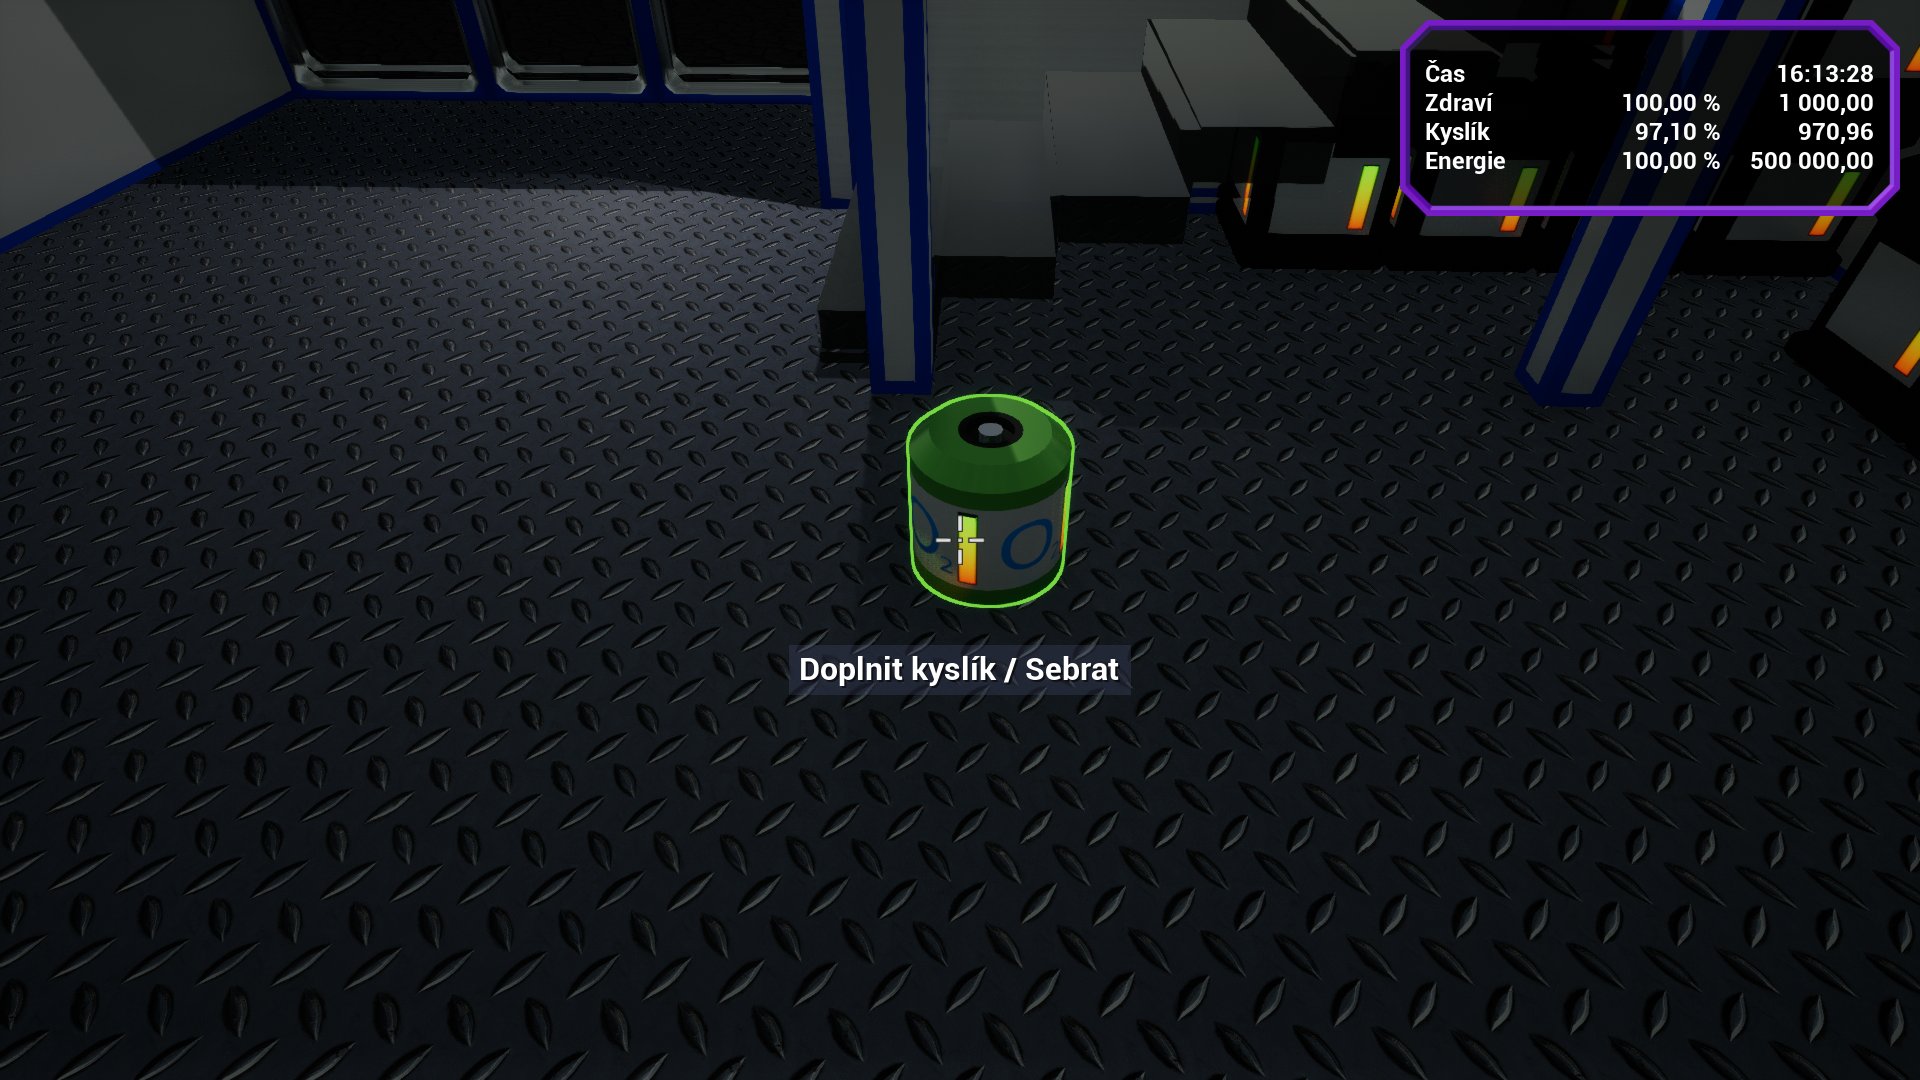
\includegraphics[ width=140mm]{../img/user/tank/0tankFull}

\caption{Umístitelné předměty -- plná kyslíková bomba}
\label{fig:user_tank_0tankFull}

\end{figure}

\FloatBarrier

Na dalším obrázku vidíme již částečně použitou kyslíkovou bombu. Pokud ji pravým tlačítkem myši sebereme a~otevřeme si inventář a~správnou skupinu (\textbf{Typ: Inventář} v~nastavení skupiny), uvidíme tento blok v~seznamu.

Požité tagy se při přidání do světa a~opětovném sebrání zachovávají.

\begin{figure}[!ht]\centering
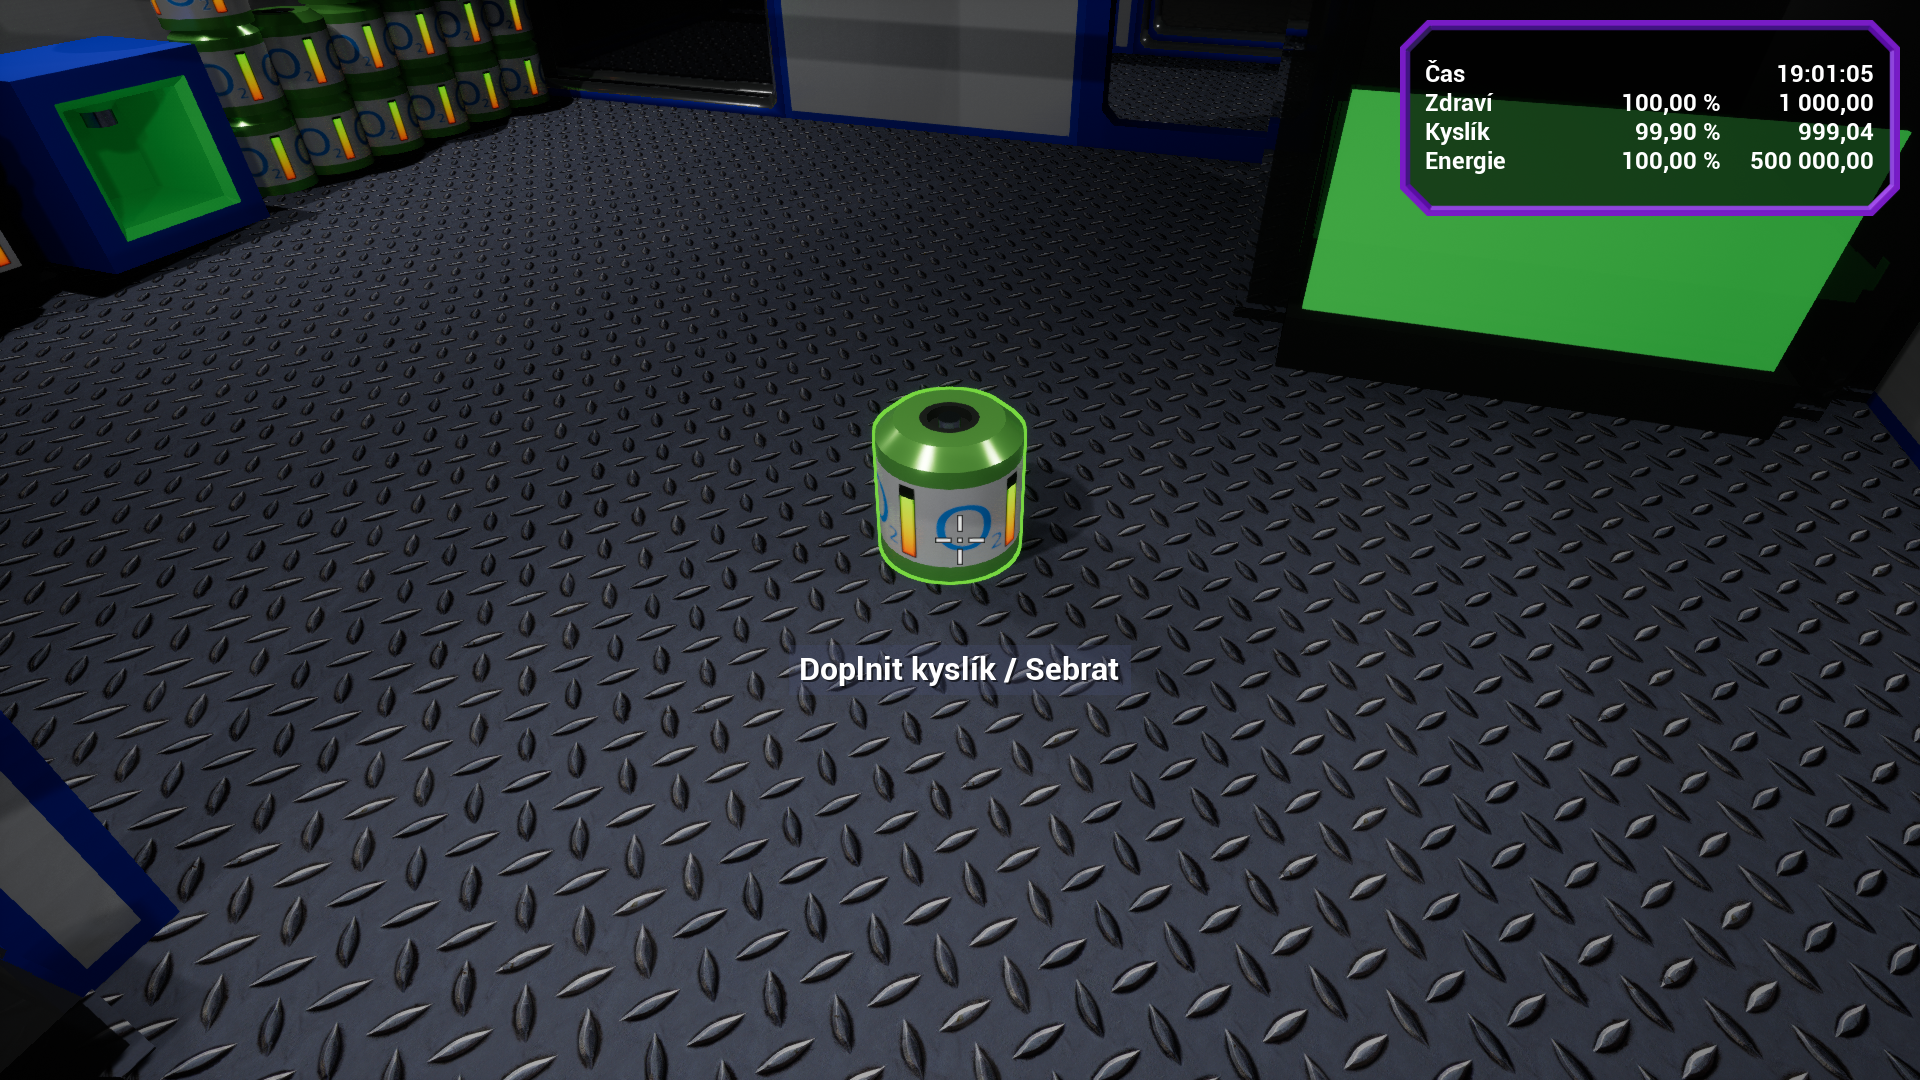
\includegraphics[ width=140mm]{../img/user/tank/1tankAfterUse}

\caption{Umístitelné předměty -- použitá bomba}
\label{fig:user_tank_1tankAfterUse}

\end{figure}

\FloatBarrier

Zároveň v~inventáři můžeme vidět přesnou hodnotu naplnění bloku.

\begin{figure}[!ht]\centering
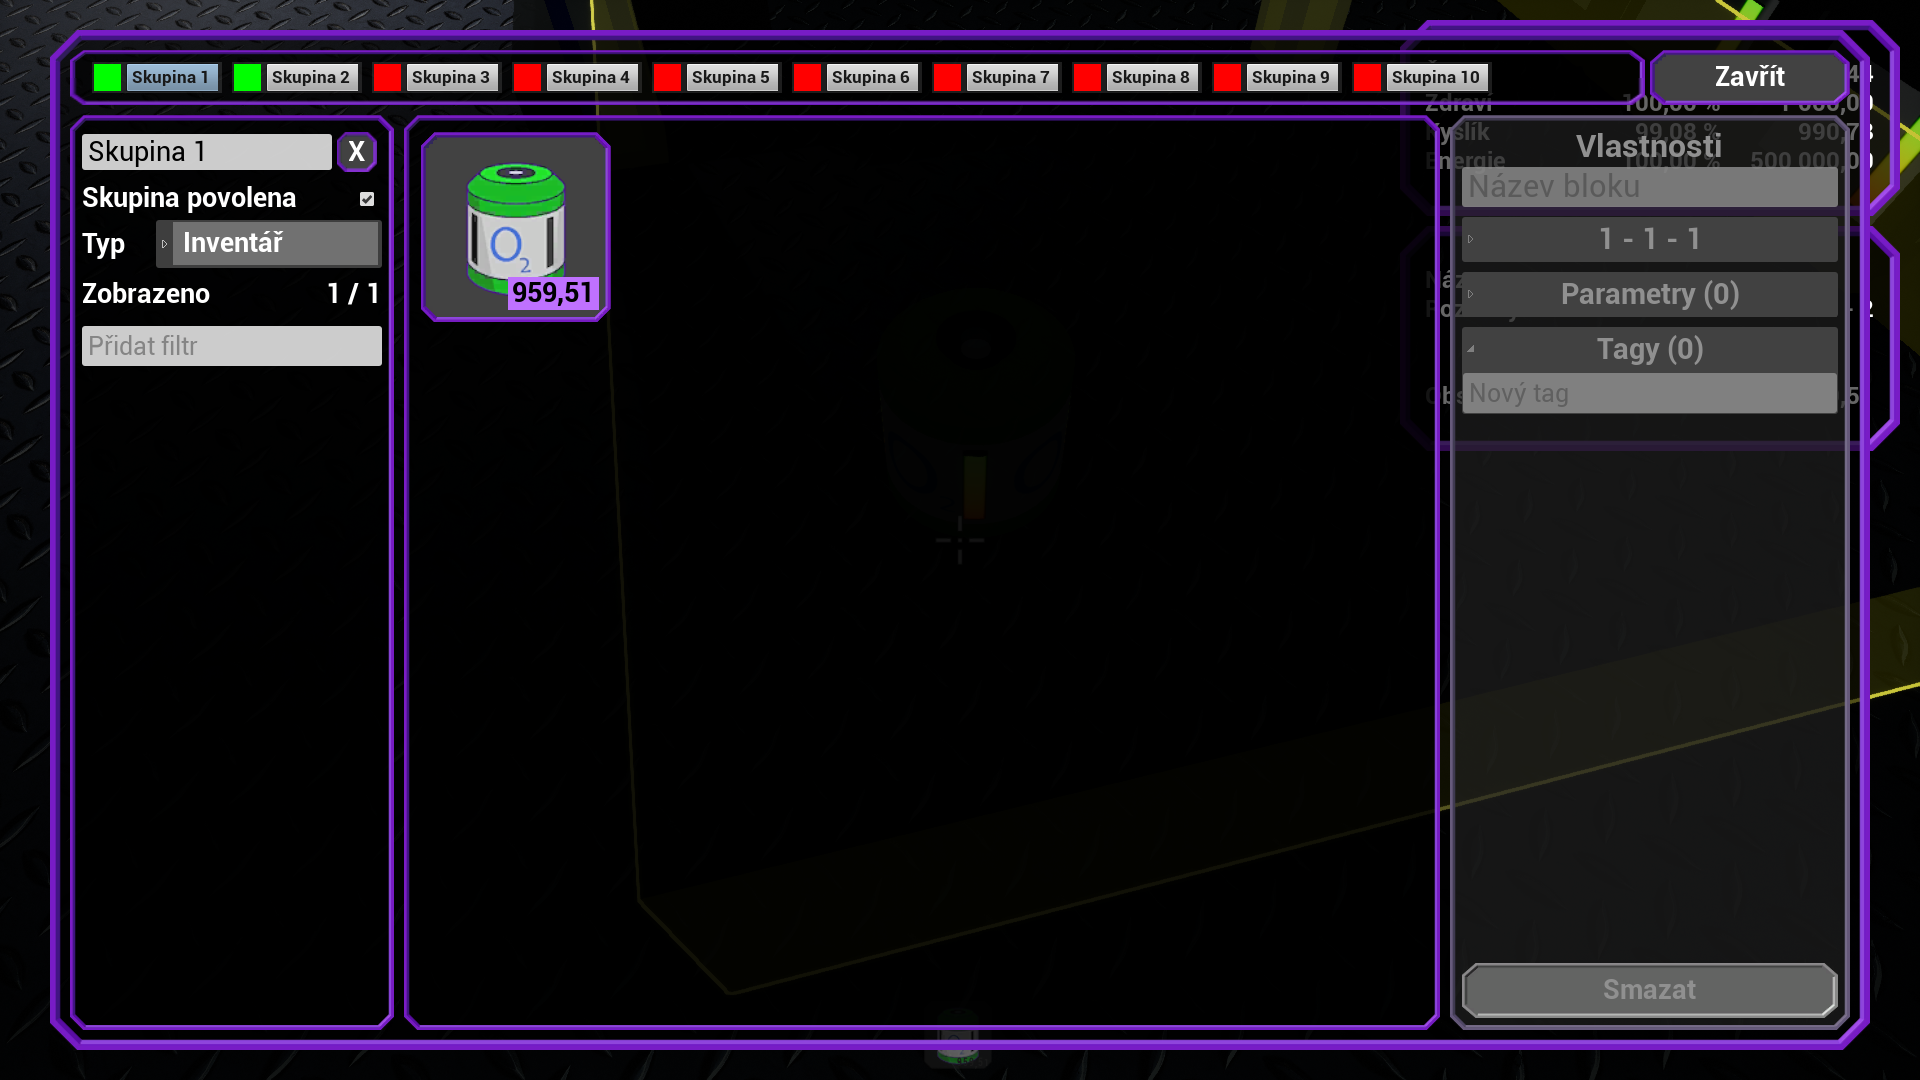
\includegraphics[ width=140mm]{../img/user/tank/2tankInventory}

\caption{Umístitelné předměty -- inventář}
\label{fig:user_tank_2tankInventory}

\end{figure}



\FloatBarrier